% Template created by Robert Maier, 2013
\documentclass[t,plaincaption]{beamer}

\mode<presentation>
{
	\usepackage{theme_cvpr/beamerthemeCVPR}
	\setbeamercovered{transparent}
}

\usepackage{verbatim}

% Use xelatex to use TTF fonts 
\usepackage{fontspec}
\setsansfont{Arial}

% set the bibliography style
%\bibliographystyle{abbrv}
\bibliographystyle{apalike}

% set document information
\def\titleEn{Joint Super-Resolution and Optical Flow Estimation}
\def\authorName{Sebastian Kümper, Philipp Krueger, Jonas Sticha}
\title[\titleEn]{\titleEn}
\author[\authorName: \titleEn]{\authorName}
\date{October 6th, 2015}

% our own used packages
\usepackage{tikz}
\usetikzlibrary{arrows, positioning}
\tikzset{
flowstyle/.style={rectangle, rounded corners, fill=TUM_lightgreenish, draw=green!40!black!80, very thick, align=left},
superstyle/.style={rectangle, rounded corners, fill=TUM_blue_5, draw=TUM_blue, very thick, align=left}
}
\usepackage{graphicx}
\usepackage{caption}
\usepackage{subcaption}
\captionsetup{compatibility=false}


\begin{document}

\frame{
\titlepage
}

\frame{
\frametitle{Outline}

\tableofcontents
}


\section{Introduction}
\frame{
\frametitle{Introduction}
\begin{itemize}
  \item Super-Resolution
  \begin{itemize}
    \item Enhance resolution of images
    \item Gain Additional Details
  \end{itemize}
\end{itemize}
}

\frame{
\frametitle{Introduction}
\begin{itemize}
  \item Super-Resolution
  \begin{itemize}
    \item Naive Upsampling
  \end{itemize}
\end{itemize}
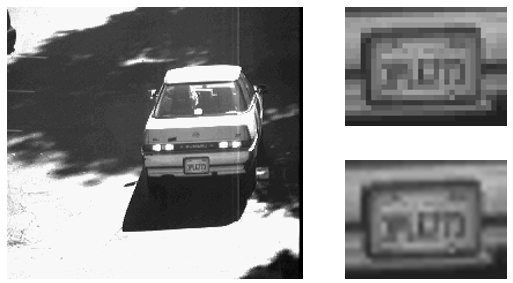
\includegraphics[width=0.9\textwidth]{images/Upscaling.png}
}

\frame{
\frametitle{Introduction}
\begin{itemize}
  \item Super-Resolution
  \begin{itemize}
    \item Using multiple images
  \end{itemize}
\end{itemize}
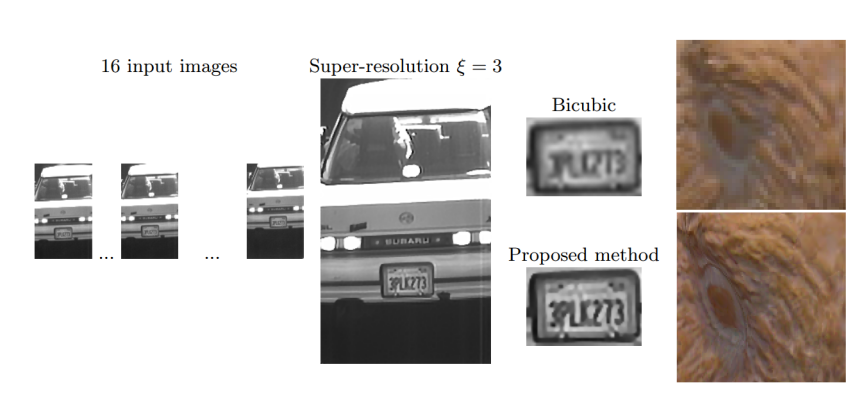
\includegraphics[width=0.9\textwidth]{images/SuperResolution.png}
\let\thefootnote\relax\footnotetext{First image: Unger, Pock, Werlberger, Bischof 2010.}

\let\thefootnote\relax\footnotetext{Second image: Goldl\"ucke, Aubry, Kolev, Cremers 2014.
}
}

\frame{
\frametitle{Introduction}
\begin{itemize}
  \item Optical Flow Estimation
  \begin{itemize}
    \item Estimate the movement in the images
  \end{itemize}
\end{itemize}
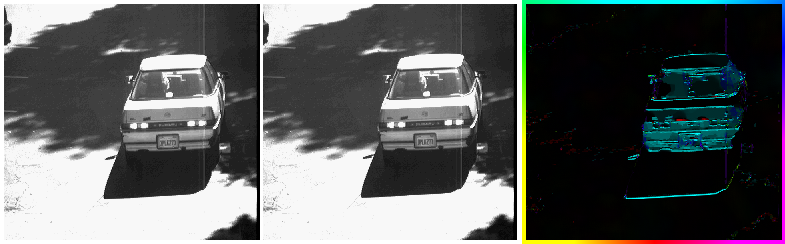
\includegraphics[width=0.9\textwidth]{images/FlowMovement.png}
}


\section{Energy Minimization Approach}
\frame{
\frametitle{Energy Minimization Approach}

\begin{columns}[T]
\column{.45\textwidth}
\begin{tikzpicture}
\tikzset{
smallImage/.style={rectangle, fill=TUM_gold, draw=TUM_orange, very thick, text width=1.5em, minimum height=2.5em, text centered},
bigImage/.style={rectangle, fill=TUM_blue_5, draw=TUM_blue, very thick, text width=2.5em, minimum height=4em, text centered},
flowField/.style={circle, fill=TUM_lightgreenish, draw=green!40!black!80, very thick, text width=1.0em, text centered},
imArrow/.style={->, >=latex', shorten >= 0.5pt, thick},
flowArrow/.style={->, >=latex', shorten >= 1pt, bend angle = 30, bend right, thick}}

\uncover<2->{
\node[text centered] (input) at (0.4, 0.8) {Input Images:};
\node[smallImage] (f1) {$f_1$};
\node[smallImage, right=1.3cm of f1] (f2) {$f_2$};
\node[smallImage, right=1.3cm of f2] (f3) {$f_3$};
\draw[imArrow] (f1.east) -- (f2.west);
\draw[imArrow] (f2.east) -- (f3.west);
}
\uncover<3->{
\node[bigImage, below=of f1] (u1) {$u_1$};
\node[bigImage, below=of f2] (u2) {$u_2$};
\node[bigImage, below=of f3] (u3) {$u_3$};
\draw[imArrow] (f1.south) -| (u1.north);
\draw[imArrow] (f2.south) -| (u2.north);
\draw[imArrow] (f3.south) -| (u3.north);
}
\uncover<4->{
\node[flowField] (v1) at (1.08, -4) {$v_1$};
\node[flowField] (v2) at (3.26, -4) {$v_2$};
\draw[flowArrow] (u1.275) to (v1.west);
\draw[flowArrow] (v1.east) to (u2.265);
\draw[flowArrow] (u2.275) to (v2.west);
\draw[flowArrow] (v2.east) to (u3.265);
}
% energy info box
\uncover<5->{
\node[rectangle, rounded corners, draw=black, thick, dashed, text width=15em, minimum height=11em] (info) at (2.17, -3.2) {};
\node[text centered] (energy) at (2.17, -4.9) {Defined by energy $E(u, v)$};
}
\end{tikzpicture}

\column{.05\textwidth}
\column{.45\textwidth}
\vspace{15mm}
\uncover<6->{
Alternating Optimization:
\begin{align*}
v^{k+1} &\leftarrow \underset{v}{\text{argmin}} ~ E(u^k, v)\\
u^{k+1} &\leftarrow \underset{u}{\text{argmin}} ~ E(u, v^{k+1})
\end{align*}
}
\end{columns}
}

\frame{
\frametitle{Flow Field Energy}
\begin{itemize}
  \setlength\itemsep{1em}
  \uncover<2->{
  \item Optical Flow Constraint: $~ u_i(x) \overset{!}{=} u_{i+1}(x + v_i(x))$}\\
  \vspace{2mm}
  \uncover<3->{$\rightarrow \text{minimize } ||u_t - \nabla u^T \cdot v||_1$}\\
  \item<4-> Total Variation: $TV(v)$
\end{itemize}
\vspace{8mm}
\uncover<5>{
\begin{center}\begin{tikzpicture}
	\node [flowstyle]{$E_{flow}(v) = \gamma ||u_t - \nabla u^T \cdot v||_1 + TV(v)$};
\end{tikzpicture}\end{center}}
}

\frame{
\frametitle{Super-Resolution Energy}
\begin{itemize}
\setlength\itemsep{1em}
  \item<2-> Super-Resolution\\
  \vspace{2mm}
  $\rightarrow \text{minimize: } ||Au - f\,||_1$
  \item<3-> Optical Flow Contraint\\
  \vspace{2mm}
  $\rightarrow \text{minimize: } ||u_t - \nabla u^T \cdot v||_1$
  \item<4-> Total Variation: $TV(u)$
\end{itemize}
\vspace{3mm}
\uncover<5->{
\begin{center}\begin{tikzpicture}
\node [superstyle]{
$E_{super}(u) = \alpha ||Au - f\,||_1 + \beta TV(u) + \gamma||u_t - \nabla u^T \cdot v||_1$};
\end{tikzpicture}\end{center}}
}

\frame{
\frametitle{Total Energy}
\begin{center}
\begin{tikzpicture}
	\node [flowstyle]{$E_{flow}(v) = \gamma ||u_t - \nabla u^T \cdot v||_1 + TV(v)$};
\end{tikzpicture}\\
\vspace{3mm}
+\\
\vspace{4mm}
\begin{tikzpicture}
\node [superstyle]{
$E_{super}(u) = \alpha ||Au - f\,||_1 + \beta TV(u) + \gamma||u_t - \nabla u^T \cdot v||_1$};
\end{tikzpicture}
\\
\vspace{5mm}
$\downarrow$\\
\vspace{5mm}
$E(u, v) = \underbrace{\alpha ||Au - f\,||_1 + \beta TV(u)}_{\text{Super-Resolution}} + \underbrace{TV(v)}_{\text{Flow}} + \underbrace{\gamma||u_t - \nabla u^T \cdot v||_1}_{\text{Coupling}}$
\end{center}
}


\section{Results}
\frame{
\frametitle{Results}
\begin{itemize}
  \item Optical Flow Estimation
  \begin{itemize}
    \item Live Demo ...
  \end{itemize}
\end{itemize}
\begin{figure}
  \centering
  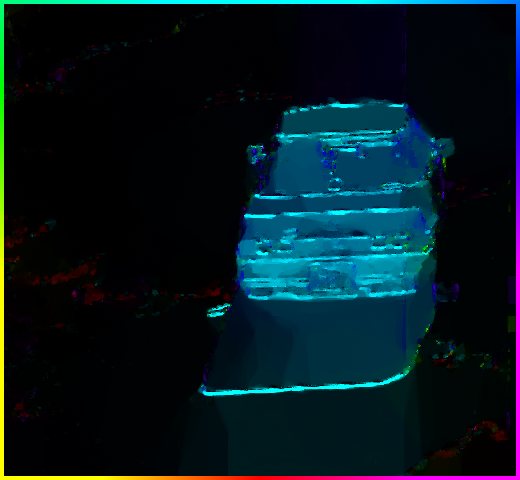
\includegraphics[width=.5\linewidth]{images/flow.png}
\end{figure}
}
\frame{
\frametitle{Results}
\begin{itemize}
  \item Super-Resolution with Optical Flow Estimation
  \begin{itemize}
    \item Input:
  \end{itemize}
\end{itemize}
\begin{figure}
\centering
\begin{subfigure}{.5\textwidth}
  \centering
  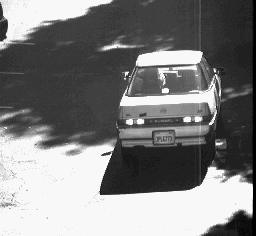
\includegraphics[width=.9\linewidth]{images/carwide_01.png}
  \caption{Input 1}
\end{subfigure}%
\begin{subfigure}{.5\textwidth}
  \centering
  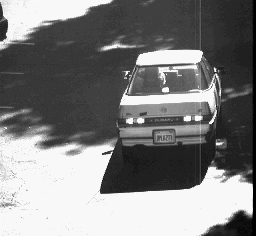
\includegraphics[width=.9\linewidth]{images/carwide_02.png}
  \caption{Input 2}
\end{subfigure}
\end{figure}
}
\frame{
\frametitle{Results}
\begin{itemize}
  \item Super-Resolution with Optical Flow Estimation
  \begin{itemize}
    \item Result:
  \end{itemize}
\end{itemize}
\begin{figure}
\centering
\begin{subfigure}{.5\textwidth}
  \centering
  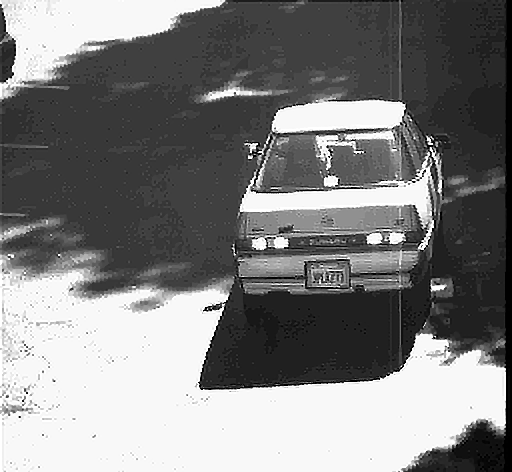
\includegraphics[width=.9\linewidth]{images/sr1.png}
  \caption{Super-Resolution 1}
\end{subfigure}%
\begin{subfigure}{.5\textwidth}
  \centering
  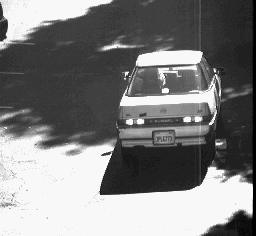
\includegraphics[width=.9\linewidth]{images/carwide_01.png}
  \caption{Input 1}
\end{subfigure}
\end{figure}
}
\frame{
\frametitle{Results}
\begin{itemize}
  \item Super-Resolution with Optical Flow Estimation
  \begin{itemize}
    \item Result zoom:
  \end{itemize}
\end{itemize}
\begin{figure}
\centering
\begin{subfigure}{.5\textwidth}
  \centering
  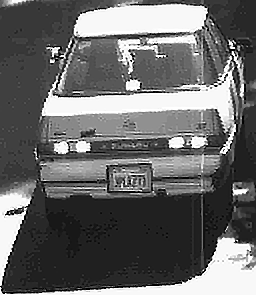
\includegraphics[width=.9\linewidth]{images/sr1_zoom.png}
  \caption{Super-Resolution 1}
\end{subfigure}%
\begin{subfigure}{.5\textwidth}
  \centering
  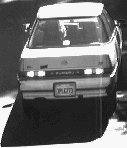
\includegraphics[width=.9\linewidth]{images/carwide_01_zoom.png}
  \caption{Input 1}
\end{subfigure}
\end{figure}
}

 
\section{Future Work}
\frame{
\frametitle{Conclusion and Future Work}
\begin{itemize}
  \item More than two input images
  \item Arbitrary scaling
  \item Optical flow estimation for movements > 1 Pixel
\end{itemize}
}

\frame{
\frametitle{End}
\begin{center}
\Huge Thank you for your attention!
\end{center}
}

\end{document}
